\documentclass[11pt]{article}

\usepackage{graphicx}
\usepackage{wrapfig}
\usepackage{url}
\usepackage{wrapfig}
\usepackage{color}
\usepackage{marvosym}
\usepackage{enumerate}
\usepackage{subfigure}
\usepackage{tikz}
\usepackage{amsmath}
\usepackage{amssymb}
\usepackage{hyperref}
\usepackage{bbm}


\oddsidemargin 0mm
\evensidemargin 5mm
\topmargin -20mm
\textheight 240mm
\textwidth 160mm



\newcommand{\vwi}{{\bf w}_i}
\newcommand{\vw}{{\bf w}}
\newcommand{\vx}{{\bf x}}
\newcommand{\vy}{{\bf y}}
\newcommand{\vxi}{{\bf x}_i}
\newcommand{\yi}{y_i}
\newcommand{\vxj}{{\bf x}_j}
\newcommand{\vxn}{{\bf x}_n}
\newcommand{\yj}{y_j}
\newcommand{\ai}{\alpha_i}
\newcommand{\aj}{\alpha_j}
\newcommand{\X}{{\bf X}}
\newcommand{\Y}{{\bf Y}}
\newcommand{\vz}{{\bf z}}
\newcommand{\msigma}{{\bf \Sigma}}
\newcommand{\vmu}{{\bf \mu}}
\newcommand{\vmuk}{{\bf \mu}_k}
\newcommand{\msigmak}{{\bf \Sigma}_k}
\newcommand{\vmuj}{{\bf \mu}_j}
\newcommand{\msigmaj}{{\bf \Sigma}_j}
\newcommand{\pij}{\pi_j}
\newcommand{\pik}{\pi_k}
\newcommand{\D}{\mathcal{D}}
\newcommand{\el}{\mathcal{L}}
\newcommand{\N}{\mathcal{N}}
\newcommand{\vxij}{{\bf x}_{ij}}
\newcommand{\vt}{{\bf t}}
\newcommand{\yh}{\hat{y}}
\newcommand{\code}[1]{{\footnotesize \tt #1}}
\newcommand{\alphai}{\alpha_i}

\pagestyle{myheadings}
\markboth{Homework 4}{Spring 2018 CS 475 Machine Learning: Homework 4}


\title{CS 475 Machine Learning: Homework 4\\Clustering, EM, Dimensionality Reduction, Graphical Models\\
	\Large{Due: Friday April 27, 2018, 11:59pm}\\
	125 Points Total \hspace{1cm} Version 1.0}
\author{}
\date{}

\begin{document}
	\large
	\maketitle
	\thispagestyle{headings}
	
	\vspace{-.5in}
	
	{\bf Make sure to read from start to finish before beginning the assignment.}
\section{Programming (65 points)}

In this assignment you will implement two variants of the $K$-means clustering algorithm, $\lambda$-means clustering and the stochastic k-means algorithm.

\subsection{$\lambda$-Means}
The $K$-means clustering algorithm groups instances into $K$ clusters. Each cluster is represented by a prototype vector $\vmuk$, which represents the mean of the examples in that cluster. Cluster assignments are ``hard,'' meaning that an instance can belong to only a single cluster at a time.

The $K$-means algorithm works by assigning instances to the cluster whose prototype $\vmuk$ has the smallest distance to the instance (based on, for example, Euclidean distance). The mean vectors $\vmuk$ are then updated based on the new assignments of instances to clusters, and this process is repeated using an EM-style iterative algorithm.

A limitation of $K$-means is that we must choose the number of clusters $K$ in advance, which can be difficult in practice. There is a variant of $K$-means called $\lambda$-means where the number of clusters can change as the algorithm proceeds. This algorithm is very similar to $K$-means but with one key difference: an instance $\vxi$ is assigned to the nearest existing cluster {\bf unless} all of the cluster prototypes have a distance larger than some threshold $\lambda$. In that case, $\vxi$ is assigned to a new cluster (cluster $K+1$ if we previously had $K$ clusters). The prototype vector for the new cluster is simply the same vector as the instance, $\vmu_{K+1} = \vxi$.
The idea here is that if an instance is not similar enough to any of the existing clusters, we should start a new one.\footnote{This algorithm (called ``DP-means'' here) is described in: B. Kulis and M.I. Jordan. Revisiting k-means: New Algorithms via Bayesian Nonparametrics. 29th International Conference on Machine Learning (ICML), 2012.}


\subsubsection{Implementation}

Your \code{LambdaMeans} class should inherit from \code{Model}, as you have done all semester. You will still implement the \code{fit} and \code{predict} methods. However, the behavior will be slightly different than in previous projects.

In unsupervised learning, the learner does not have access to labeled data. However, the datasets you have been using contain labels in the training data. You should not use these labels at all during learning. Additionally, since the clustering algorithm cannot read the correct labels, we must be clear about what ``label'' you are returning with \code{predict}.

Your implementation should include the following functionality:

\begin{itemize}
\item The \code{fit} method should learn the cluster parameters based on the training examples. While the labels are available in the provided data, the clustering algorithms should not use this information. The result of the \code{fit} method are the cluster parameters: the means $\vmuk$ and the number of clusters $K$. 
\item The \code{predict} method should label the examples by assigning them to the closest cluster.
The value of the label should be the cluster index, i.e., an example closest to $k$th cluster should receive label $k$. While this document will describe the algorithm as if $k$ is in the set $\{1,\ldots,K\}$, it is fine for your code to use the set $\{0,\ldots,K-1\}$ because the evaluation scripts (see Section 1.8) will give the same results whether you use 0-indexing or 1-indexing.
\end{itemize}

\subsection{Inference with EM}
\label{sec:EM}
The $K$-means algorithm and the $\lambda$-means algorithm are based on an EM-style iterative approach. On each iteration, the algorithm computes 1 E-step and 1 M-step.

In the E-step, cluster assignments $r_{nk}$ are determined based on the current model parameters $\vmuk$. 
$r_{nk}$ is an {\bf indicator} variable that is 1 if the $n$th instance belongs to cluster $k$ and 0 otherwise.

Suppose there are currently $K$ clusters. You should set the indicator variable for these clusters as follows. For $k \in \{1,\ldots,K\}$:

\begin{equation}
\label{eq:E1}
r_{nk} =  \left\{
     \begin{array}{lr}
        1~~  \textrm{if} ~~  k = \arg\min_j ||\vxn - \vmuj||_2  \textrm{ and }  \min_j ||\vxn - \vmuj||_2 \leq \lambda \\
        0 ~~   ~~ \textrm{otherwise}
     \end{array}
   \right.
\end{equation}

\noindent where $||\vx-\vx'||_2$ denotes the Euclidean distance, $\sqrt {\sum_{f=1}^m (x_f - x'_f)^2}$. When computing this distance, assume that if a feature is not present in an instance $\vx$, then it has value 0.

Additionally, you must consider the possibility that the instance $\vxn$ is assigned to a new cluster, $K+1$. The indicator for this is:

\begin{equation}
\label{eq:E2}
r_{n,K+1} =  \left\{
     \begin{array}{lr}
        1 ~~  \textrm{if} ~~  \min_j ||\vxn - \vmuj||_2 > \lambda \\
        0 ~~    ~~ \textrm{otherwise}
     \end{array}
   \right.
\end{equation}

\noindent If $r_{n,K+1}=1$, you should immediately set $\vmu_{K+1}=\vxn$ and $K=K+1$, before moving on to the next instance $\vx_{n+1}$. You should not wait until the M-step to update $\vmu_{K+1}$.

{\bf Be sure to  iterate through the instances in the order they appear in the dataset.}

After the E-step, you will update the mean vectors $\vmuk$ for each cluster $k \in \{1,\ldots,K\}$ (where $K$ may have increased during the E-step). This forms the M-step, in which the model parameters $\vmuk$ are updated using the new cluster assignments:

\begin{equation}
\vmu_{k}= \frac{\sum_n r_{nk} \vxn}{\sum_n r_{nk}}
\end{equation}

\noindent This process will be repeated for a given number of iterations (see Section 1.6).

\subsection{Cluster Initialization}
\label{sec:initial}
As we discussed in class, clustering objectives are non-convex. Therefore, different initializations will lead to different clustering solutions. In order for us to test the submitted code, we must have everyone use the same initialization method.

In $K$-means, the standard initialization method is to randomly place each instance into one of the $K$ clusters. However, in $\lambda$-means you can initialize the algorithm with only one cluster ($K=1$). You should initialize the prototype vector to the mean of all instances: $\vmu_1 = \bar{\vx} = \frac{1}{N} \sum_{n=1}^{N} \vxn$.

\subsection{Lambda Value}

The default value of $\lambda$ will be the average distance from each training instance to the mean of the training data:

\begin{equation}
\label{eq:default}
\lambda^{\textrm{\scriptsize (default)}} =  \frac{1}{N} \sum_{i=1}^{N} ||\vxi-\bar{\vx}||_2,   
\end{equation}

\noindent where $\bar{\vx}$ is the mean vector of the training instances (also the initialization of $\vmu_1$ in \ref{sec:initial}).

You \emph{must} add a command line argument to allow this value to be adjusted via the command line.  Do this by
adding the following to the \code{get\_args} function in \code{classify.py}:
	\begin{footnotesize}
		\begin{verbatim}
		parser.add_argument("--cluster_lambda", type=float, 
		help="The value of lambda in lambda-means", default=0.0)
		\end{verbatim}
	\end{footnotesize}

How you implement the $\lambda$ value is up to you, but it probably makes more sense to set its value in your \code{LambdaMeans} rather than in \code{get\_args}. You can do this by setting the input value to 0 by default (as in the above code example), then setting the value to the default in Eq. \ref{eq:default} if the value passed to the \code{fit} function is 0. You can assume that any value we supply through the command line will be $>0$.

We highly encourage you to experiment with different values of $\lambda$ to see how it affects the number of clusters that are produced.

\subsection{Stochastic K-means}
The Stochastic K-means algorithm (SKA) associates the data point $\vxi$ to a cluster based on a probability distribution that depends on the distance between the data point and the cluster centers. SKA is less dependent than K-means on the initial cluster choices.

The cluster initialization is the same as that of the K-means algorithm. (See section \ref{sec:initial}). At the beginning of each iteration, assign each data point $\vxn$ to the closest mean. You should set the indicator variable for the $K$ clusters as follows. For $k \in \{1,\ldots,K\}$,

%\begin{equation}
%\label{eq:E4}
%r_{nk} =  \left\{
%     \begin{array}{lr}
%        1~~  \textrm{if} ~~  k = \arg\min_j ||\vxn - \vmuj||_2  \\
%        0 ~~   ~~ \textrm{otherwise}
%     \end{array}
%   \right.
%\end{equation}

\begin{equation}
\label{eq:E4}
r_{nk} =  \left\{
     \begin{array}{lr}
        1~~  \textrm{if} ~~  k = \arg\min_j d(\vxn, \vmuj)  \\
        0 ~~   ~~ \textrm{otherwise}
     \end{array}
   \right.
\end{equation}

\noindent The probability that $\vxn$ belongs to cluster $k$ is defined as follows:

\begin{equation}
\label{eq:E5}
%p_{nk}^{(i)} =  \frac{e^{-\beta^{(i)}\frac{d(x_n,\mu_k)}{\hat{d}(x_n)}}}{\sum_{j=1}^{K} e^{-\beta^{(i)}\frac{d(x_n,\mu_k)}{\hat{d}(x_n)}} }
p_{nk}^{(i)} =  \frac{\exp\left(\frac{-\beta^{(i)}d(x_n,\mu_k)}{\hat{d}(x_n)}\right)}{\sum_{j=1}^{K} \exp\left(\frac{-\beta^{(i)}d(x_n,\mu_k)}{\hat{d}(x_n)}\right) }
\end{equation}

\noindent where $d(\vxn,\vmuk)$ is the Euclidean distance between $\vxn$ and $\vmuk$ and $\hat{d}(\vxn)$ is the mean Euclidean distance between $\vxn$ and all $\vmuk$, $k \in \{1,\ldots,K\}$

\begin{equation}
\hat{d}(\vxn)= \frac{1}{K}\sum_{k=1}^{K}\vert\vert \vxn - \vmuk \vert\vert_2
\end{equation}

\noindent The model parameters $\mu_k$ should then be updated as

\begin{equation}
\vmu_{k}= \frac{\sum_n p_{nk} \vxn}{\sum_n p_{nk}}
\end{equation}

\noindent To implement this, you should create another class that inherits from the \code{Model} class called \code{StochasticKMeans}.  Note that you will not use a $\lambda$ value for this algorithm.

% TODO: Use square Euclidean distances in eqn 4, 5? Be consistent with section \ref{sec:EM}
% TODO: Use a constant beta? Or have $\beta$ change in each iteration? Latter for now. c will be the cmd line arg in this case. Add the registeroption portion once this is decided.
\subsubsection { How to choose $\beta$}
The parameter $\beta$ increases linearly with iteration, as follows:

\begin{equation}
\beta^{(i)} = c(i-1),
\end{equation}

\noindent where $i$ is the iteration number and $c$ is a constant. You may want to experiment with different values of $c$, but use $c = 2$ in your final implementation.  Note that in the limit, as $\beta \rightarrow  \infty$, SKA behaves similarly to the K-means algorithm.

\subsection{Number of Iterations}
\label{sec:iterations}

The default number of clustering iterations is 10. An iteration is defined as computing 1 E-step and 1-M step of the algorithm (in that order).

You \emph{must} add a command line argument to allow this value to be adjusted via the command line.  Do this by
adding the following to the \code{get\_args} function in \code{classify.py}:
	\begin{footnotesize}
		\begin{verbatim}
		parser.add_argument("--clustering_training_iterations", type=int, 
		help="The number of training EM iterations")
		\end{verbatim}
	\end{footnotesize}

\subsection{Implementation Details}

\subsubsection{Tie-Breaking}
When assigning an instance to a cluster you may encounter ties, where the instance is equidistant to two or more clusters. When a tie occurs, select the cluster with the lowest cluster index.

\subsubsection{Empty Clusters}
It is possible (though unlikely) that a cluster can become empty while training the algorithm. That is, there may exist a cluster $k$ such that $r_{nk}=0,\ \forall n$. In this case, you should set $\vmuk={\mathbf 0}$. Do not remove empty clusters.

\subsubsection{Expanding the Cluster Set}
In standard $K$-means, you typically create arrays of size $K$ to store the parameters. Since the number of clusters can grow with $\lambda$-means, you will need to set up data structures that can accommodate this.
One option is to simply use arrays of a fixed size, expanding the size of the array if you run out of space (by creating a larger array and copying the contents of the old array). Alternatively, you can expand the size of the data structure as you go along (though this will likely run slower).


\subsection{Evaluation}
\label{sec:evaluation}

For clustering we cannot simply use accuracy against true labels to evaluate the output, since your prediction outputs are simply the indices of clusters (which could be arbitrary).  Instead we will evaluate your output using an information-theoretic metric called {\em variation of information} (VI), which can be used to measure the dependence of the cluster indices with the true labels.
The variation of information between two random variables $Y$ and $\hat{Y}$ is defined as: $H(Y|\hat{Y}) + H(\hat{Y}|Y)$. Lower is better. This will have a value of 0 if there is a one-to-one mapping between the two labelings, which is the best you can do.
We have provided a python script to compute this metric: \code{cluster\_accuracy.py}.  Additionally, we have provided a script that displays the number of unique clusters: \code{number\_clusters.py}.

We will evaluate your implementation on the standard data sets you have been using (\code{speech}, \code{bio}, etc.) as well as the three-class \code{Iris} dataset, included here.  We have removed the \code{nlp} data set from this assignment for computational efficiency.	
	
\section{Analytical (60 points)}
	
\paragraph{1) Clustering (14 points)}
	
We want to cluster the data set $\vx_1,\ldots,\vx_n$ using the K-means algorithm. The K-means algorithm partitions the $n$ observations into $k$ sets ($k < n$) $\mathbf{S} = \{S_1, S_2, \ldots, S_k\}$ so as to minimize the within-cluster sum of squares:
\begin{eqnarray*}
\mathop{\textrm{argmin}}_{\mathbf{S}=\{S_1,\ldots,S_k\}}\sum_{j=1}^k\sum_{\vxi\in S_j}\|\vx_i-\mu_j\|_2^2
\end{eqnarray*}
where $\mu_j$ is the mean of the examples in $S_j$.

\begin{enumerate}[(a)]
\item Prove that the objective is non-increasing after each E/M step.
\item One variant is called K-medoids. K-medoids is similar to K-means: both K-means and K-medoids minimize the squared error. However, unlike K-means, K-medoids chooses a training example as a cluster center (medoid). It is more robust to noise and outliers as compared to k-means because it minimizes a sum of pairwise dissimilarities instead of a sum of squared Euclidean distances. 

Give an example to illustrate that K-medoids will be more robust to outliers than K-means.
\item Another variant of K-means is to change the distance metric to the L1 distance, which is more robust to outliers. In this case, we are minimizing:
\begin{align}
\min_{S=\{S_1,...,S_k\}}\sum_{j=1}^k\sum_{\vxi\in S_j}\|\vx_j-\mu_j\|_1
\end{align}
where $\mu_j$ is the center of $S_j$ w.r.t. to L1 distance. It turns out that computing the medians is involved when computing the cluster center. That is why this algorithm is call K-medians. Does the cluster center have to be an actual instance from the dataset? Explain why.
\end{enumerate}
	
\paragraph{2) Expectation-Maximization (12 points)} 

As we discussed in class, clustering objectives are non-convex. Therefore, different initializations will lead to different clustering solutions.

As an example, take Gaussian mixture model (GMM) clustering. Suppose all the parameters of the GMM are initialized such that all components/clusters have the same mean $\mu_k=\hat{\mu}$ and same covariance $\Sigma_k=\hat{\Sigma}$ for all $k=1,\ldots,K$.
\begin{enumerate}[(a)]
\item Prove that the EM
algorithm will converge after a single iteration for any choice of the initial mixing coefficients $\pi$.
\item Show that this solution has the property $\mu_k=\frac{1}{N}\sum_{n=1}^{N}\mathbf{x}_n$ and $\Sigma_k=\frac{1}{N}\sum_{n=1}^{N}(\mathbf{x}_n-\mu_k)(\mathbf{x}_n-\mu_k)^T$, where $N$ is the total number of examples. Note that this represents a degenerate case of the mixture model in which all of the components are identical, and in practice we try to avoid such solutions by using an appropriate initialization.
\end{enumerate}

\paragraph{3) Dimensionality Reduction (9 points)}

Show that in the limit $\sigma^2 \rightarrow 0$, the posterior mean for the probabilistic PCA model becomes an orthogonal projection onto the principal subspace, as in conventional PCA.
	

\paragraph{4) Probabilistic PCA (10 points)}

Draw a directed probabilistic graphical model representing a discrete mixture of probabilistic PCA models in which each PCA model has its own values of $\mathbf{W}$, $\boldsymbol{\mu}$, and $\sigma^2$. Then draw a modified graph in which these parameter values are shared between the components of the mixture. The graph should represent the model for a single data point $\mathbf{x}$. (Hint: refer to slide 24 of the Dimensionality Reduction lecture as a starting point.)
	

\paragraph{5) Graphical Models (15 points)}
	
	Consider the Bayesian Network given in Figure \ref{fig:bn}. Are the sets ${\bf A}$ and ${\bf B}$ d-separated given set ${\bf C}$ for each of the following definitions of ${\bf A}$, ${\bf B}$ and ${\bf C}$? Justify each answer.
\begin{figure}[h]
	\begin{center}
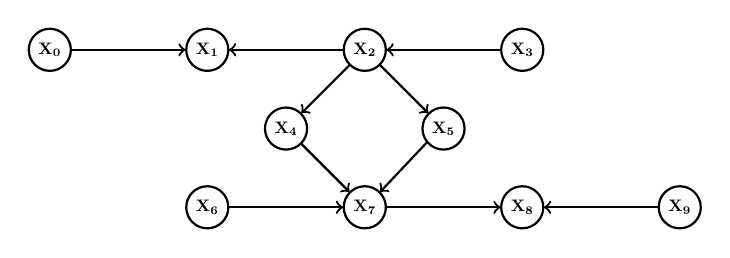
\begin{tikzpicture}[style=thick,scale=1] 
\newcommand{\nsize}{.6}
\begin{scope}[shape=circle,minimum size=0.1cm] 
\tikzstyle{every node}=[draw,fill] 
\node[fill=none,scale=\nsize] (X_0) at (-2,2) {$\mathbf{X_0}$};
\node[fill=none,scale=\nsize] (X_1) at (0,2) {$\mathbf{X_1}$};
\node[fill=none,scale=\nsize] (X_2) at (2,2) {$\mathbf{X_2}$};
\node[fill=none,scale=\nsize] (X_3) at (4,2) {$\mathbf{X_3}$};
\node[fill=none,scale=\nsize] (X_4) at (1,1) {$\mathbf{X_4}$};
\node[fill=none,scale=\nsize] (X_5) at (3,1) {$\mathbf{X_5}$};
\node[fill=none,scale=\nsize] (X_6) at (0,0) {$\mathbf{X_6}$};
\node[fill=none,scale=\nsize] (X_7) at (2,0) {$\mathbf{X_7}$};
\node[fill=none,scale=\nsize] (X_8) at (4,0) {$\mathbf{X_8}$};
\node[fill=none,scale=\nsize] (X_9) at (6,0) {$\mathbf{X_9}$};
\draw [->] (X_0) -- (X_1);
\draw [->] (X_2) -- (X_1);
\draw [->] (X_3) -- (X_2);
\draw [->] (X_2) -- (X_4);
\draw [->] (X_2) -- (X_5);
\draw [->] (X_4) -- (X_7);
\draw [->] (X_5) -- (X_7);
\draw [->] (X_6) -- (X_7);
\draw [->] (X_7) -- (X_8);
\draw [->] (X_9) -- (X_8);
\end{scope} 
\end{tikzpicture}
		\caption{A directed graph}
			\label{fig:bn}
		\end{center}
\end{figure}\\
\begin{enumerate}[a.]
\item ${\bf A} = \{ X_3 \}$, ${\bf B} = \{ X_4 \}$, ${\bf C} = \{X_1,X_2\}$
\item ${\bf A} = \{ X_5 \}$, ${\bf B} = \{X_4\}$, ${\bf C} = \{X_2,X_7\}$
\item ${\bf A} = \{X_4\}$, ${\bf B} = \{X_6\}$, ${\bf C} = \{X_8\}$
\item ${\bf A} = \{X_5\}$, ${\bf B} = \{X_4\}$, ${\bf C} = \{X_2\}$
\item ${\bf A} = \{X_6, X_9\}$, ${\bf B} = \{X_8\}$, ${\bf C} = \{X_3,X_1\}$
\end{enumerate}
Now assume that Figure 1 is a Markov Random Field, where each edge is undirected (just drop the direction of each edge.) Re-answer each of the above questions with justifications for your answers.
	
\section{What to Submit}
	You will need to create an account on gradescope.com and signup for this class. The course is \href{https://gradescope.com/courses/13142}{\url{https://gradescope.com/courses/13142}}. Use entry code {\tt 974Z3W}. See this video for instructions on how to upload a homework assignment: \href{https://www.youtube.com/watch?v=KMPoby5g_nE}{\url{https://www.youtube.com/watch?v=KMPoby5g_nE}}. In each assignment you will submit two things to gradescope.
	\begin{enumerate}
		\item \textbf{Submit your code (.py files) to gradescope.com as a zip file}. \textbf{Your code must be uploaded as code.zip with your code in the root directory}. By `in the root directory,' we mean that the zip should contain \texttt{*.py} at the root (\texttt{./*.py}) and not in any sort of substructure (for example \texttt{hw4/*.py}). One simple way to achieve this is to zip using the command line, where you include files directly (e.g., \texttt{*.py}) rather than specifying a folder (e.g., \texttt{hw4}):
		\begin{verbatim}
		zip code.zip *.py
		\end{verbatim}
		
		We will run your code using the exact command lines described earlier, so make sure it works ahead of time, and make sure that it doesn't crash when you run it on the test data. Remember to submit all of the source code, including what we have provided to you. We will include {\tt requirements.txt} but nothing else.
		\item \textbf{Submit your writeup to gradescope.com}. \textbf{Your writeup must be compiled from latex and uploaded as a PDF}. It should contain all of the answers to the analytical questions asked in the assignment. Make sure to include your name in the writeup PDF and to use the provided latex template for your answers. 
	\end{enumerate}
	
	\section{Questions?}
	Remember to submit questions about the assignment to the appropriate group on Piazza: \href{https://piazza.com/class/jatranyaky957s}{\url{https://piazza.com/class/jatranyaky957s}}.
	
\end{document}